\section{Life Cycle Of Software}
\subsection{Whats's Life Cycle Of Software?}
As the name suggest it's the life cycle of a software from start to finish , life cycle also known as model is a methodology
that serves to help developers in building their product , each life cycle has steps and a chronology to follow
\subsection{WaterFall Life Cycle}
\subsubsection{First Version}
\vspace{0.5cm}
\begin{center}
\begin{tikzpicture}
    \draw (-1,0) rectangle (3.5,1.5);
    \node at (1.25,0.75) {Definition \& Needs Analysis};

   \draw[->] (3.5,0.75) -- (5,0.75) -- (5,0);

    \draw (4,-1.5) rectangle (6,0);
    \node at (5,-0.75) {Conception};

    \draw[->] (6,-0.75) -- (7.5,-0.75) -- (7.5,-1.5);

    \draw (6.5,-3) rectangle (8.5,-1.5);
    \node at (7.5,-2.25) {Coding};

    \draw[->] (8.5,-2.25) -- (10,-2.25) -- (10,-3);

    \draw (9,-4.5) rectangle (11,-3);
    \node at (10,-3.75) {Testing};

    \draw[->] (11,-3.75) -- (13.75,-3.75) -- (13.75,-4.5);

    \draw (11.5,-6) rectangle (16,-4.5);
    \node at (13.75,-5.25) {Deployment \& Maintenance};
\end{tikzpicture}
\end{center}
\subsubsection{Improved Version}
\vspace{0.5cm}
\begin{center}
\begin{tikzpicture}
    \draw (-1,0) rectangle (3.5,1.5);
    \node at (1.25,0.75) {Definition \& Needs Analysis};

   \draw[->] (3.5,0.75) -- (5,0.75) -- (5,0);

    \draw (4,-1.5) rectangle (6,0);
    \node at (5,-0.5) {Achitectural};
    \node at (5,-1){Design};
    \draw (4,-3) rectangle (6,-1.5);
    \node at (5,-2) {Detailed};
    \node at (5,-2.5) {Design};

    \draw[->] (6,-1.5) -- (7.5,-1.5) -- (7.5,-2);

    \draw (6.5,-3.5) rectangle (8.5,-2);
    \node at (7.5,-2.75) {Coding};

    \draw[->] (8.5,-2.25) -- (10,-2.25) -- (10,-3);

    \draw (9,-4.5) rectangle (11,-3);
    \node at (10,-3.75) {Unit Test};
    \draw (9,-6) rectangle (11,-4.5);
    \node at (10,-5) {Integration};
    \node at (10,-5.5) {Test};

    \draw[->] (11,-4.5) -- (13.75,-4.5) -- (13.75,-5);

    \draw (11.5,-6.5) rectangle (16,-5);
    \node at (13.75,-5.75) {Deployment \& Maintenance};
\end{tikzpicture}
\end{center}
\subsection{V Life Cycle}
\vspace{1cm}
\begin{center}
\begin{tikzpicture}
    \draw (-1,0) rectangle (3.5,1.5);
    \node at (1.25,0.75) {Definition \& Needs Analysis};

    \draw[->] (3.5,0.75) -- (12.5,0.75);
    \draw[->] (1.25,0) -- (2.75,-0.75);

    \draw (1,-2) rectangle (4.5,-0.75);
    \node at (2.75,-1.375) {Architectural Design};

    \draw[->] (4.5,-1.375) -- (10.5,-1.375);
    \draw[->] (2.75,-2) -- (4.75,-2.75);

    \draw (3,-4) rectangle (6.5,-2.75);
    \node at (4.75,-3.375) {Detailed Design};

    \draw[->] (6.5,-3.375) -- (8.5,-3.375);
    \draw[->] (4.75,-4) -- (7.5,-5.25);
    
    \draw (6.45,-6.5) rectangle (8.5,-5.25);
    \node at (7.5,-5.875) {Coding};

    \draw[->] (7.5,-5.25) -- (10.25,-4);
    
    \draw (8.5,-4) rectangle (12,-2.75);
    \node at (10.25,-3.375) {Unit Test};

    \draw[->] (10.25,-2.75) -- (12.25,-2);
    
    \draw (10.5,-2) rectangle (14,-0.75);
    \node at (12.25,-1.375) {Integration Test};

    \draw[->] (12.25,-0.75) -- (14.5,0);
    
    \draw (12.5,0) rectangle (16.5,1.5);
    \node at (14.5,0.75) {Acceptation Test};


\end{tikzpicture}
\end{center}
\subsection{Prototyping Life Cycle}
\vspace{1cm}
\begin{center}
    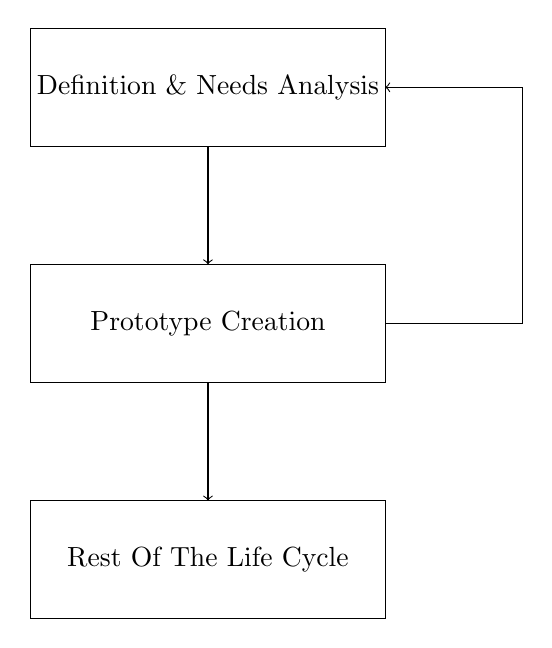
\begin{tikzpicture}
    \draw (-1,0) rectangle (3.5,1.5);
    \node at (1.25,0.75) {Definition \& Needs Analysis};
 
    \draw[->] (1.25,0) -- (1.25,-1.5);

    \draw (-1,-3) rectangle (3.5,-1.5);
    \node at (1.25,-2.25) {Prototype Creation};

    \draw[->] (3.5,-2.25) -- (5.25,-2.25) -- (5.25,0.75) -- (3.5,0.75);
    \draw[->] (1.25,-3) -- (1.25,-4.5);
     
    \draw (-1,-6) rectangle (3.5,-4.5);
    \node at (1.25,-5.25) {Rest Of The Life Cycle};



    \end{tikzpicture}
\end{center}
\subsection{Incremental Life Cycle}

\vspace{2cm}
\begin{center}
    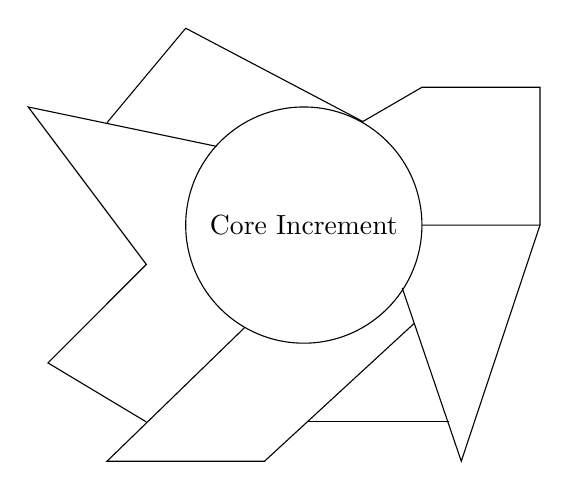
\begin{tikzpicture}
        \draw (0,0) circle[radius = 1.5cm] node {Core Increment};
        \draw (1.5,0) -- (3,0) -- (2,-3) -- (1.25,-0.8);
        \draw (0.75,1.315) -- (-1.5,2.5) -- (-2.5,1.3);
        \draw (1.4,-1.25) -- (-0.5,-3) -- (-2.5,-3) -- (-0.75,-1.3);
        \draw (0.050,-2.5) -- (1.85,-2.5); 
        \draw (3,0) -- (3,1.75) -- (1.5,1.75) -- (0.75,1.315);
        \draw (-2,-2.5) -- (-3.25,-1.75) -- (-2,-0.5) -- (-3.5 , 1.5) -- (-1.11,1);
    \end{tikzpicture}
\end{center}
\subsection{Spiral Life Cycle}
\begin{center}
\begin{tikzpicture}
   \draw[->] (-6,0) -- (6,0);
    \draw[->] (0,-6) -- (0,6);

    \draw[domain=0:6.28*5, variable=\t, samples=500, smooth] 
        plot ({\t r}: {0.15*\t});
\end{tikzpicture}
\end{center}
\subsection{Hybrid Life Cycle}
\vspace{4cm}
   \begin{tikzpicture}
    \draw (2.5,0) rectangle (7,1.5);
    \node at (4.75,0.75) {The Project};
   
    \draw [->] (4.75,0) -- (4.75 , - 1.5) -- (4.75 , -2.5);
    \draw [->] (4.75,-1.5) -- (-4.75,-1.5) -- (-4.75,-2.5);
    \draw [->] (4.75 , -1.5) -- (14.75,-1.5) -- (14.75,-2.5);

    \draw (-6,-4) rectangle (-3.5,-2.5);
    \node at (-4.75,-3.25) {Part$_{1}$};

    \draw (-6,-9) rectangle (-3.5,-7.5);
    \node at (-4.75,-8.25) {Life Cycle$_{1}$};

    \draw[dash pattern=on 1pt off 3pt, line width=1pt] (-2.75,-3.25) -- (2.75,-3.25);

    \draw (3.5,-4) rectangle (6,-2.5);
    \node at (4.75,-3.25) {Part$_{5}$};
    
    \draw (3.5,-9) rectangle (6,-7.5);
    \node at (4.75,-8.25) {Life Cycle$_{5}$};


    \draw[dash pattern=on 1pt off 3pt, line width=1pt] (6.75,-3.25) -- (12.75,-3.25);

    \draw (13.5,-4) rectangle (16,-2.5); 
    \node at (14.75,-3.25) {Part$_{n}$};
   
    \draw (13.5,-9) rectangle (16,-7.5);
    \node at (14.75,-8.25) {Life Cycle$_{n}$};


\end{tikzpicture}
